\documentclass[12pt,a4paper]{article}
% 基础包
\usepackage{ctex}
\usepackage{geometry}
\usepackage{fancyhdr}
\usepackage{lastpage}
\usepackage{indentfirst}
% 字体设置
\usepackage{mathptmx}
\usepackage[T1]{fontenc}
% 数学公式
\usepackage{amsmath,amssymb,amsfonts}
\usepackage{mathtools}
\usepackage{nccmath}
\everymath{\displaystyle}
\usepackage{txfonts}
\providecommand{\varparallel}{\mathrel{/\!/}}
% 表格
\usepackage{array}
\usepackage{booktabs}
\usepackage{multirow}
\usepackage{colortbl}
% 图片和颜色
\usepackage{graphicx}
\usepackage{xcolor}
\usepackage{caption}
\usepackage{subcaption}
% 列表
\usepackage{enumitem}
\usepackage{tasks}
% TikZ 画图
\usepackage{tikz}
\usepackage{tikz-3dplot}
\usetikzlibrary{
	arrows.meta, calc, patterns, intersections,
	through, angles, quotes, decorations.pathmorphing
}
% 页面设置
\geometry{
	left=1.6cm,
	right=2.04cm,
	top=1.6cm,
	bottom=2.54cm,
	headheight=1.2cm,
	footskip=0.8cm,
	nohead
}
% 行距和段落
\linespread{1.5}
\setlength{\parindent}{2em}
\setlength{\parskip}{0.5ex}
% 页脚设置
\pagestyle{fancy}
\fancyhf{}
\fancyfoot[C]{\makebox[0pt][c]{数学试题~第\thepage 页（共\pageref{LastPage}页）}}
\renewcommand{\headrulewidth}{0pt}
\renewcommand{\footrulewidth}{0pt}
% 选择题选项环境
\NewTasksEnvironment[
label=\Alph*.,
label-width=1.5em,
item-indent=2em,
column-sep=2em,
before-skip=0.8em,
after-skip=0.8em
]{choicesFour}[\choice](4)

\NewTasksEnvironment[
label=\Alph*.,
label-width=1.5em,
item-indent=2em,
column-sep=3em,
before-skip=0.8em,
after-skip=0.8em
]{choicesTwo}[\choice](2)

\NewTasksEnvironment[
label=\Alph*.,
label-width=1.5em,
item-indent=2em,
before-skip=0.8em,
after-skip=0.8em
]{choicesOne}[\choice](1)

\begin{document}
	
	\noindent {\large\bfseries 绝密$\bigstar$启用前}
	\vspace*{0.5cm}
	
	\begin{center}
		{\Large 2026年普通高等学校招生全国统一考试}\\[0.8cm]
		{\LARGE\bfseries 数~~~~学\ （答案解析版）}
	\end{center}
	
	\noindent 本试卷共4页，19小题，满分150分，考试时间120分钟.
	
	\vspace{0.3cm}
	
	\noindent\hangindent=2em {\bfseries 一、选择题：本题共8小题，每小题5分，共40分.}
	
	\begin{enumerate}[leftmargin=*,label=\arabic*.,itemsep=0.8ex]
		
		\item 样本数据$6,8,4,5,12$的中位数为
		\begin{choicesFour}
			\choice $5$ \choice $6$ \choice $8$ \choice $9$
		\end{choicesFour}
		\textbf{【答案】B}\\
		\textbf{【解析】}排序为$4,5,6,8,12$，中位数为$6$.
		
		\item 已知平面向量$\boldsymbol{a},\boldsymbol{b}$不共线，且$2\boldsymbol{a}+y\boldsymbol{b}=x\boldsymbol{a}-3\boldsymbol{b}$，则
		\begin{choicesFour}
			\choice $x=2,\ y=-3$ \choice $x=-2,\ y=3$ \choice $x=2,\ y=3$ \choice $x=-2,\ y=-3$
		\end{choicesFour}
		\textbf{【答案】A}\\
		\textbf{【解析】}因$\boldsymbol a,\boldsymbol b$不共线，比较系数得$x=2,\ y=-3$.
		
		\item 已知集合
		\[
		A=\left\{\sin\frac{7\pi}{3},\ \cos\frac{5\pi}{4},\ \tan\frac{5\pi}{4}\right\},\qquad
		B=\left[-\frac{\sqrt3}{2},-\frac12\right],
		\]
		则$A\cap B=$
		\begin{choicesFour}
			\choice $\left\{-\dfrac{\sqrt2}{2}\right\}$
			\choice $\left\{\dfrac{\sqrt3}{2}\right\}$
			\choice $\{1\}$
			\choice $\varnothing$
		\end{choicesFour}
		\textbf{【答案】A}\\
		\textbf{【解析】}
		\[
		\sin\frac{7\pi}{3}=\frac{\sqrt3}{2},\quad
		\cos\frac{5\pi}{4}=-\frac{\sqrt2}{2},\quad
		\tan\frac{5\pi}{4}=1.
		\]
		其中只有$-\dfrac{\sqrt2}{2}\in B$，故$A\cap B=\left\{-\dfrac{\sqrt2}{2}\right\}$.
		
		\item 曲线$y=5x+8\ln x$在点$(1,5)$处的切线方程为
		\begin{choicesFour}
			\choice $y=3x+2$ \choice $y=5x$ \choice $y=8x-3$ \choice $y=13x-8$
		\end{choicesFour}
		\textbf{【答案】D}\\
		\textbf{【解析】}$y'=5+\dfrac8x$，在$x=1$处斜率为$13$，切线为$y-5=13(x-1)$，即$y=13x-8$.
		
		\item 已知抛物线$C_1:y^2=2p_1x\ (p_1>0)$和$C_2:x^2=2p_2y\ (p_2>0)$均经过点$(4,8)$，则$C_1$的焦点与$C_2$的焦点之间的距离为
		\begin{choicesFour}
			\choice $12$ \choice $4\sqrt5$ \choice $6$ \choice $\dfrac{\sqrt{65}}{2}$
		\end{choicesFour}
		\textbf{【答案】D}\\
		\textbf{【解析】}代入$(4,8)$得$p_1=8,\ p_2=1$. 焦点分别为$(4,0)$与$\left(0,\dfrac12\right)$，距离为
		\[
		\sqrt{4^2+\left(\frac12\right)^2}=\frac{\sqrt{65}}2.
		\]
		
		\item 已知函数$f(x)=\dfrac{x+2}{e^x+a}$的最大值为$1$，则$a=$
		\begin{choicesFour}
			\choice $\dfrac12$ \choice $1$ \choice $\dfrac32$ \choice $2$
		\end{choicesFour}
		\textbf{【答案】B}\\
		\textbf{【解析】}最大值为$1$，需$x+2\le e^x+a$恒成立，即$a\ge x+2-e^x$. 设$g(x)=x+2-e^x$，则$g'(x)=1-e^x$，最大值为$g(0)=1$，故$a=1$.
		
		\item 一百零八塔位于宁夏回族自治区青铜峡市，其独特的建筑格局和深远的历史文化闻名遐迩. 该塔群共有$108$座塔，依山势自上而下排成$12$行，将第$i$行中塔的座数记为$a_i\ (i=1,2,\dots,12)$. 其中$a_1=1$，$a_2=a_3=3$，$a_4=a_5=5$，且$a_6,a_7,\dots,a_{12}$是一个首项为$7$，公差为$2$的等差数列. 将$a_1,a_2,\dots,a_{12}$分为$6$组，每组$2$个数，使得每组的$2$个数之和可构成一个项数为$6$且公差为$d\ (d>0)$的等差数列，则$d=$
		\begin{choicesFour}
			\choice $2$ \choice $4$ \choice $6$ \choice $8$
		\end{choicesFour}
		\textbf{【答案】B}\\
		\textbf{【解析】}数列为
		\[
		1,3,3,5,5,7,9,11,13,15,17,19.
		\]
		总和为$108$，若$6$个两两和构成等差数列，则中间平均数为$18$. 经验证$d=4$时可分组为
		\[
		(1,7),(3,9),(3,13),(5,15),(5,19),(11,17),
		\]
		和为$8,12,16,20,24,28$，公差为$4$.
		
		\item 设
		\[
		U=\{(x_1,x_2,x_3)\mid x_i\in\{-2,-1,1,2\},\ i=1,2,3\}
		\]
		为空间中$64$个点构成的集合，点$P(1,1,1)$，记样本空间$\Omega=U\setminus\{P\}$. 从$\Omega$中随机取一个点，定义随机变量$X$如下：对$\Omega$中的每个点$A(x_1,x_2,x_3)$，令$X(A)=x_1+x_2+x_3$，则$X$的数学期望为
		\begin{choicesFour}
			\choice $-\dfrac1{21}$ \choice $-\dfrac1{63}$ \choice $0$ \choice $\dfrac17$
		\end{choicesFour}
		\textbf{【答案】A}\\
		\textbf{【解析】}全体$64$个点坐标和总和为$0$. 去掉$P(1,1,1)$后，总和为$-3$，共有$63$个点，故期望为$-\dfrac3{63}=-\dfrac1{21}$.
		
	\end{enumerate}
	
	\vspace{0.3cm}
	
	\noindent\hangindent=2em {\bfseries 二、选择题：本题共3小题，每小题6分，共18分.}
	
	\begin{enumerate}[leftmargin=*,label=\arabic*.,resume,itemsep=0.8ex]
		
		\item 设$z=3+2\mathrm{i}$，则
		\begin{choicesTwo}
			\choice $\overline{z}=3-2\mathrm{i}$
			\choice $|z|=5$
			\choice $z^2=5+12\mathrm{i}$
			\choice $\dfrac{z+3}{z-1}\in\mathbb{R}$
		\end{choicesTwo}
		\textbf{【答案】AC}\\
		\textbf{【解析】}$\overline z=3-2\mathrm i$，A正确；$|z|=\sqrt{13}$，B错误；$z^2=(3+2\mathrm i)^2=5+12\mathrm i$，C正确；
		\[
		\frac{z+3}{z-1}=\frac{6+2\mathrm i}{2+2\mathrm i}=2-\mathrm i,
		\]
		不是实数，D错误.
		
		\item 在空间中，$A,B$为两个定点，动点$C$到直线$AB$的距离为$2$，动点$D$到直线$AB$的距离为$1$. 若二面角$C-AB-D$为$60^\circ$，则
		\begin{choicesOne}
			\choice $\angle CAD\ge60^\circ$
			\choice $CD\ge\sqrt3$
			\choice 当$AB\perp CD$时，$CD\perp$平面$ABD$
			\choice 当$AB\perp$平面$ACD$时，$AC\perp AD$
		\end{choicesOne}
		\textbf{【答案】BC}\\
		\textbf{【解析】}以$AB$为$x$轴建立坐标系，设$C,D$在垂直于$AB$的平面内投影向量长分别为$2,1$，夹角$60^\circ$. 则
		\[
		CD^2=(x_C-x_D)^2+2^2+1^2-2\cdot2\cdot1\cos60^\circ
		=(x_C-x_D)^2+3\ge3,
		\]
		故B正确. 当$AB\perp CD$时，$x_C=x_D$，可验证$CD$与平面$ABD$内两条相交直线垂直，故C正确.
		
		\item 已知圆$C_1:(x+1)^2+y^2=1$，圆$C_2:(x-1)^2+y^2=1$，圆$C_3:x^2+(y-\sqrt3)^2=1$. 直线$l:y=kx+b$与$C_1,C_2,C_3$均有两个交点，记$l$被$C_1,C_2,C_3$截得的弦长分别为$s_1,s_2,s_3$，则
		\begin{choicesOne}
			\choice $k$可以取任意实数
			\choice 满足$s_1=s_2=s_3$的直线$l$共有$3$条
			\choice 满足$s_1+s_2+s_3=3$的直线$l$多于$3$条
			\choice 当$b=0$时，$s_1+s_2+s_3$的最大值为$\dfrac{2\sqrt{21}}{3}$
		\end{choicesOne}
		\textbf{【答案】BCD}\\
		\textbf{【解析】}三圆圆心构成边长为$2$的等边三角形.
		
		A错误：例如$k=\dfrac1{\sqrt3}$时，无法找到使三圆均相交于两点的$b$.
		
		B正确：弦长相等要求三圆心到直线距离相等. 设直线为$ax+by+c=0$且$a^2+b^2=1$，由到$C_1,C_2$距离相等得$ac=0$. 分$c=0$与$a=0$讨论，可得三条直线.
		
		C正确：除B中三条外，由连续性及对称性还存在其他直线使$s_1+s_2+s_3=3$，故多于$3$条.
		
		D正确：当$b=0$时，设直线为$y=kx$，则
		\[
		s_1+s_2+s_3=\frac{4+2\sqrt{k^2-2}}{\sqrt{k^2+1}},\quad |k|>\sqrt2.
		\]
		令$u=\sqrt{k^2-2}\ge0$，则
		\[
		s_1+s_2+s_3=2\cdot\frac{2+u}{\sqrt{u^2+3}},
		\]
		最大值为$\dfrac{2\sqrt{21}}3$.
		
	\end{enumerate}
	
	\vspace{0.3cm}
	
	\noindent {\bfseries 三、填空题：本题共3小题，每小题5分，共15分.}
	
	\begin{enumerate}[leftmargin=*,label=\arabic*.,resume,itemsep=0.8ex]
		
		\item 双曲线$5x^2-6y^2=1$的离心率为\underline{\quad$\dfrac{\sqrt{66}}6$\quad}.\\
		\textbf{【解析】}化为标准形式
		\[
		\frac{x^2}{1/5}-\frac{y^2}{1/6}=1.
		\]
		故$a^2=\dfrac15,\ b^2=\dfrac16$，
		\[
		e=\frac ca=\sqrt{\frac{a^2+b^2}{a^2}}
		=\sqrt{\frac{1/5+1/6}{1/5}}=\sqrt{\frac{11}{6}}=\frac{\sqrt{66}}6.
		\]
		
		\item 已知$f(x)=2\sin(\omega x+\theta)\ (\omega\in\mathbb{Z},\ 0\le\theta<2\pi)$是偶函数，$f(x)$在区间$\left(0,\dfrac{\pi}{2}\right)$单调递增，则$\theta=$\underline{\quad$\dfrac{3\pi}{2}$\quad}，$f\left(\dfrac{2\pi}{3}\right)=$\underline{\quad$1$\quad}.\\
		\textbf{【解析】}偶函数要求$\cos\theta=0$，故$\theta=\dfrac\pi2$或$\dfrac{3\pi}2$. 当$\theta=\dfrac{3\pi}2$时，$f(x)=-2\cos(\omega x)$，可取$\omega=\pm1,\pm2$使其在$\left(0,\dfrac\pi2\right)$递增. 此时
		\[
		f\left(\frac{2\pi}3\right)=-2\cos\frac{2\pi}3=1.
		\]
		
		\item  设实数$q$满足：存在数列$\{a_n\}$，使得对于任意$n\in\mathbb{N}^*$，均有$a_1+a_2+\cdots+a_n=n^2+n$，且$\{a_n\}$中有某连续$9$项$a_k,a_{k+1},\dots,a_{k+8}$是公比为$q$的等比数列，则$q$的最大值为\underline{\quad 不存在\quad}.\\
		\textbf{【解析】}由$S_n=n^2+n$得
		\[
		a_n=S_n-S_{n-1}=2n.
		\]
		因此任意连续三项为$2k,2(k+1),2(k+2)$. 若成等比数列，则需
		\[
		[2(k+1)]^2=(2k)[2(k+2)],
		\]
		即$(k+1)^2=k(k+2)$，矛盾. 故按题干条件不存在这样的实数$q$.
		
	\end{enumerate}
	
	\vspace{0.3cm}
	
	\noindent {\bfseries 四、解答题：本题共5小题，共77分.}
	
	\begin{enumerate}[leftmargin=*,label=\arabic*.,resume,itemsep=1.2ex]
		
		\item (13分)\\
		\noindent\begin{minipage}[t]{0.7\linewidth}
			如图，在直三棱柱$ABC-A_1B_1C_1$中，$\angle ACB=90^\circ$，$AC=BC$，$D,E$分别为$AB,AC_1$的中点.
			
			(1) 证明：$DE\varparallel$平面$BCC_1B_1$；
			
			(2) 设$CC_1=2$，直线$DE$与平面$ACC_1A_1$所成的角为$45^\circ$，求直线$DE$到平面$BCC_1B_1$的距离.
		\end{minipage}%
		\begin{minipage}[t]{0.3\linewidth}
			\centering
			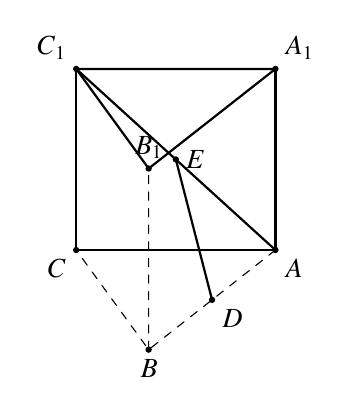
\begin{tikzpicture}[baseline=(current bounding box.north), scale=1.15, line cap=round, line join=round]
				\coordinate (C) at (0,0);
				\coordinate (A) at (2.2,0);
				\coordinate (B) at (0.8,-1.1);
				\coordinate (C1) at (0,2);
				\coordinate (A1) at (2.2,2);
				\coordinate (B1) at (0.8,0.9);
				\coordinate (D) at ($(A)!0.5!(B)$);
				\coordinate (E) at ($(A)!0.5!(C1)$);
				
				\draw[dashed] (A)--(B)--(C) (B)--(B1);
				\draw[thick] (A)--(C);
				\draw[thick] (A1)--(B1)--(C1)--cycle;
				\draw[thick] (A)--(A1) (C)--(C1);
				\draw[thick] (A)--(C1);
				\draw[thick] (D)--(E);
				
				\fill (C) circle(1pt) node[below left]{$C$};
				\fill (A) circle(1pt) node[below right]{$A$};
				\fill (B) circle(1pt) node[below]{$B$};
				\fill (D) circle(1pt) node[below right]{$D$};
				\fill (C1) circle(1pt) node[above left]{$C_1$};
				\fill (A1) circle(1pt) node[above right]{$A_1$};
				\fill (B1) circle(1pt) node[above]{$B_1$};
				\fill (E) circle(1pt) node[right]{$E$};
			\end{tikzpicture}
		\end{minipage}
		
		\textbf{【解析】}
		
		(1) 在$\triangle ABC_1$中，$D$为$AB$中点，$E$为$AC_1$中点，故$DE\varparallel BC_1$. 又$BC_1\subset$平面$BCC_1B_1$，所以$DE\varparallel$平面$BCC_1B_1$.
		
		(2) 设$AC=BC=a$，以$C$为原点，$CA,CB,CC_1$方向为坐标轴建立空间直角坐标系，则
		\[
		A(a,0,0),\quad B(0,a,0),\quad C_1(0,0,2),
		\]
		\[
		D\left(\frac a2,\frac a2,0\right),\quad E\left(\frac a2,0,1\right).
		\]
		于是
		\[
		\overrightarrow{DE}=\left(0,-\frac a2,1\right).
		\]
		平面$ACC_1A_1$为$y=0$，其法向量为$(0,1,0)$. 直线$DE$与该平面所成角$\theta$满足
		\[
		\sin\theta=\frac{\left|\overrightarrow{DE}\cdot(0,1,0)\right|}{|\overrightarrow{DE}|}
		=\frac{a/2}{\sqrt{a^2/4+1}}.
		\]
		由$\theta=45^\circ$，得
		\[
		\frac{a/2}{\sqrt{a^2/4+1}}=\frac{\sqrt2}{2},
		\]
		解得$a=2$.
		
		平面$BCC_1B_1$为$x=0$，直线$DE$上各点$x$坐标均为$1$，故直线到该平面的距离为
		\[
		\boxed{1}.
		\]
		
		\item (15分)\\
		已知在$\triangle ABC$中，$AB=3$，$BC=2\sqrt3$，$\cos B=\dfrac{\sqrt3}{3}$.
		
		(1) 求$\cos A$；
		
		(2) 设$D,E$两点满足：$D$在$BA$的延长线上，$DE\varparallel BC$，$AE\perp AC$. 若$DE=\sqrt6$，求$CE$.
		
		\textbf{【解析】}
		
		(1) 由余弦定理，
		\[
		AC^2=AB^2+BC^2-2\cdot AB\cdot BC\cos B
		=9+12-2\cdot3\cdot2\sqrt3\cdot\frac{\sqrt3}{3}=9.
		\]
		故$AC=3$. 再由余弦定理，
		\[
		\cos A=\frac{AB^2+AC^2-BC^2}{2\cdot AB\cdot AC}
		=\frac{9+9-12}{18}=\frac13.
		\]
		所以
		\[
		\boxed{\cos A=\frac13}.
		\]
		
		(2) 以$A$为原点，$AC$所在直线为$x$轴建立平面直角坐标系，则
		\[
		A(0,0),\quad C(3,0).
		\]
		由$\cos A=\dfrac13$，$\sin A=\dfrac{2\sqrt2}{3}$，且$AB=3$，可取
		\[
		B(1,2\sqrt2).
		\]
		设$D$在$BA$延长线上，则$D=-tB=(-t,-2\sqrt2t)$，$t>0$.
		
		因为$AE\perp AC$，所以$E$在$y$轴上，设$E(0,y)$.
		
		又$DE\varparallel BC$，而
		\[
		\overrightarrow{BC}=(2,-2\sqrt2),
		\]
		故存在$\lambda$使
		\[
		\overrightarrow{DE}=(t,y+2\sqrt2t)=\lambda(2,-2\sqrt2).
		\]
		由$t=2\lambda$得$\lambda=\dfrac t2$，于是
		\[
		y+2\sqrt2t=-\sqrt2t,
		\]
		即
		\[
		y=-3\sqrt2t.
		\]
		又
		\[
		DE=|\lambda|\cdot BC=\frac t2\cdot2\sqrt3=t\sqrt3.
		\]
		由$DE=\sqrt6$，得$t=\sqrt2$. 因此
		\[
		E(0,-6).
		\]
		于是
		\[
		CE=\sqrt{(3-0)^2+(0+6)^2}=3\sqrt5.
		\]
		所以
		\[
		\boxed{CE=3\sqrt5}.
		\]
		
		\item (15分)\\
		设整数$N\ge2$. 某同学用一个球进行投篮练习，至多投篮$N$次，当且仅当投中1次时或$N$次均未投中时，停止练习. 设该同学每次投中的概率为$p\ (0<p<1)$，各次投中与否相互独立. 记$X$为停止练习时该同学的投篮次数.
		
		(1) 当$N=4,\ p=\dfrac13$时，求$X$的分布列；
		
		(2) 设$k,m$均为自然数.
		
		\hspace*{2em}(i) 当$k\le N-1$时，求$P(X>k)$；
		
		\hspace*{2em}(ii) 当$k+m\le N-1$时，证明：$P(X>k+m\mid X>k)=P(X>m)$.
		
		\textbf{【解析】}
		
		(1) 当$X=1,2,3$时，表示第$1,2,3$次首次投中；当$X=4$时，表示前三次均未投中. 故
		\[
		P(X=1)=\frac13,
		\]
		\[
		P(X=2)=\frac23\cdot\frac13=\frac29,
		\]
		\[
		P(X=3)=\left(\frac23\right)^2\cdot\frac13=\frac4{27},
		\]
		\[
		P(X=4)=\left(\frac23\right)^3=\frac8{27}.
		\]
		分布列为
		\[
		\begin{array}{c|cccc}
			X & 1 & 2 & 3 & 4\\ \hline
			P & \dfrac13 & \dfrac29 & \dfrac4{27} & \dfrac8{27}
		\end{array}
		\]
		
		(2)(i) $X>k$表示前$k$次均未投中，因此
		\[
		\boxed{P(X>k)=(1-p)^k}.
		\]
		
		(ii) 当$k+m\le N-1$时，由(i)得
		\[
		P(X>k+m)=(1-p)^{k+m},\qquad P(X>k)=(1-p)^k.
		\]
		所以
		\[
		P(X>k+m\mid X>k)
		=\frac{P(X>k+m)}{P(X>k)}
		=\frac{(1-p)^{k+m}}{(1-p)^k}
		=(1-p)^m
		=P(X>m).
		\]
		证毕.
		
		\item (17分)\\
		已知椭圆$C:\dfrac{x^2}{a^2}+\dfrac{y^2}{b^2}=1\ (a>b>0)$的左焦点为$F(-1,0)$，离心率为$\dfrac12$.
		
		(1) 求$C$的方程；
		
		(2) 设$O$为坐标原点，过$F$且斜率大于$0$的动直线$l$与$C$交于$P,Q$两点，其中$Q$在第三象限，直线$PO$与$C$的另一个交点为$R$.
		
		\hspace*{2em}(i) 若$\triangle PQR$的面积是$\triangle PFO$的面积的$3$倍，求$l$的方程；
		
		\hspace*{2em}(ii) 求$\tan\angle PQR$的最小值.
		
		\textbf{【解析】}
		
		(1) 左焦点为$(-1,0)$，故$c=1$. 又离心率$e=\dfrac ca=\dfrac12$，所以$a=2$，
		\[
		b^2=a^2-c^2=4-1=3.
		\]
		椭圆方程为
		\[
		\boxed{\frac{x^2}{4}+\frac{y^2}{3}=1}.
		\]
		
		(2) 设直线$l:y=t(x+1)$，其中$t>0$. 令$u=x+1$，则$x=u-1$，代入椭圆方程：
		\[
		\frac{(u-1)^2}{4}+\frac{t^2u^2}{3}=1.
		\]
		整理得
		\[
		(3+4t^2)u^2-6u-9=0.
		\]
		设两根为$u_P>0,\ u_Q<0$，分别对应$P,Q$.
		
		(i) 因为$R$是直线$PO$与椭圆的另一交点，椭圆关于原点对称，所以$R=-P$.
		
		直线$l$上两点$P,Q$满足
		\[
		P=(u_P-1,tu_P),\quad Q=(u_Q-1,tu_Q).
		\]
		于是
		\[
		S_{\triangle PQR}=|P\times Q|=t(u_P-u_Q).
		\]
		又
		\[
		S_{\triangle PFO}=\frac12|y_P|=\frac12tu_P.
		\]
		由题意，
		\[
		t(u_P-u_Q)=3\cdot\frac12tu_P,
		\]
		即
		\[
		u_P-u_Q=\frac32u_P,
		\]
		故
		\[
		u_P=-2u_Q.
		\]
		由根与系数关系，
		\[
		u_P+u_Q=\frac6{3+4t^2},\qquad u_Pu_Q=-\frac9{3+4t^2}.
		\]
		代入$u_P=-2u_Q$，得
		\[
		-u_Q=\frac6{3+4t^2},
		\]
		且
		\[
		-2u_Q^2=-\frac9{3+4t^2}.
		\]
		消去$u_Q$，得
		\[
		3+4t^2=8,
		\]
		所以
		\[
		t^2=\frac54,\quad t=\frac{\sqrt5}{2}.
		\]
		故直线$l$的方程为
		\[
		\boxed{y=\frac{\sqrt5}{2}(x+1)}.
		\]
		
		(ii) 仍设$u_P,u_Q$为上述方程两根，记
		\[
		S=u_P+u_Q=\frac6{3+4t^2}.
		\]
		向量
		\[
		\overrightarrow{QP}=(u_P-u_Q,t(u_P-u_Q)),
		\]
		\[
		\overrightarrow{QR}=(-P)-Q=(2-S,-tS).
		\]
		于是
		\[
		|\overrightarrow{QP}\times\overrightarrow{QR}|=2t(u_P-u_Q),
		\]
		\[
		\overrightarrow{QP}\cdot\overrightarrow{QR}
		=(u_P-u_Q)\left[2-S(1+t^2)\right].
		\]
		因此
		\[
		\tan\angle PQR
		=\frac{2t}{2-S(1+t^2)}.
		\]
		代入$S=\dfrac6{3+4t^2}$，化简得
		\[
		\tan\angle PQR
		=\frac{3+4t^2}{t}
		=4t+\frac3t.
		\]
		由均值不等式，
		\[
		4t+\frac3t\ge2\sqrt{12}=4\sqrt3,
		\]
		当且仅当$4t=\dfrac3t$，即$t=\dfrac{\sqrt3}{2}$时取等号.
		
		所以
		\[
		\boxed{\tan\angle PQR_{\min}=4\sqrt3}.
		\]
		
		\item (17分)\\
		已知函数$f(x)$的定义域为$\mathbb{R}$，且当$x<0$时，$f(x)=2^x$. 对任意$x_0\in\mathbb{R}$，定义集合
		\[
		D(x_0)=\{d\in\mathbb{R}\mid f(x_0+d)>f(x_0)\}.
		\]
		
		(1) 若当$x\ge0$时，$f(x)=1-x$，求$D(-1)$；
		
		(2) 若$f(x)$是奇函数，$f(x_1)\le f(x_2)$，且$x_1x_2\ne0$，证明：$D(x_2)\subseteq D(x_1)$；
		
		(3) 设$f(x)$满足：① 若$f(x_1)\le f(x_2)$，则$D(x_2)\subseteq D(x_1)$；② 当$0<x<1$时，$f(x)<f(0)$.
		
		\hspace*{2em}(i) 证明：$f(0)\ge1$；
		
		\hspace*{2em}(ii) 证明：$f(x)$在区间$(0,+\infty)$单调递增.
		
		\textbf{【解析】}
		
		(1) $f(-1)=2^{-1}=\dfrac12$. 令$x=-1+d$.
		
		若$x<0$，即$d<1$，则
		\[
		f(x)=2^x>\frac12\iff x>-1\iff d>0.
		\]
		得$0<d<1$.
		
		若$x\ge0$，即$d\ge1$，则
		\[
		f(x)=1-x>\frac12\iff x<\frac12\iff d<\frac32.
		\]
		得$1\le d<\dfrac32$.
		
		综上，
		\[
		\boxed{D(-1)=\left(0,\frac32\right)}.
		\]
		
		(2) 因$f$为奇函数，且$x<0$时$f(x)=2^x$，故
		\[
		f(0)=0,
		\]
		且当$x>0$时，
		\[
		f(x)=-f(-x)=-2^{-x}.
		\]
		于是可分别求得：
		\[
		x<0\Rightarrow D(x)=(0,-x),
		\]
		\[
		x>0\Rightarrow D(x)=(-\infty,-x]\cup(0,+\infty).
		\]
		
		若$f(x_1)\le f(x_2)$且$x_1x_2\ne0$，分情况讨论：
		
		当$x_1,x_2<0$时，$2^{x_1}\le2^{x_2}$，故$x_1\le x_2$，从而$-x_1\ge -x_2$，于是
		\[
		D(x_2)=(0,-x_2)\subseteq(0,-x_1)=D(x_1).
		\]
		
		当$x_1,x_2>0$时，$-2^{-x_1}\le-2^{-x_2}$，故$x_1\le x_2$，从而$-x_2\le -x_1$，于是
		\[
		D(x_2)=(-\infty,-x_2]\cup(0,+\infty)
		\subseteq(-\infty,-x_1]\cup(0,+\infty)=D(x_1).
		\]
		
		当$x_1>0,x_2<0$时，$f(x_1)<0<f(x_2)$，条件自动满足，且
		\[
		D(x_2)=(0,-x_2)\subseteq(0,+\infty)\subseteq D(x_1).
		\]
		故$D(x_2)\subseteq D(x_1)$.
		
		(3)(i) 若$f(0)<1$，因$\lim\limits_{x\to0^-}2^x=1$，可取$x\in(-1,0)$，使得
		\[
		f(x)=2^x>f(0).
		\]
		于是$f(0)\le f(x)$，由①得
		\[
		D(x)\subseteq D(0).
		\]
		又当$0<d<-x$时，$x+d<0$，且
		\[
		f(x+d)=2^{x+d}>2^x=f(x),
		\]
		故$d\in D(x)$. 取$d=-\dfrac x2$，则$0<d<1$，从而$d\in D(0)$，即
		\[
		f(d)>f(0),
		\]
		这与②矛盾. 故
		\[
		\boxed{f(0)\ge1}.
		\]
		
		(ii) 先证：当$0<x<1$时，$f(x)<1$.
		
		若存在$0<x<1$使$f(x)\ge1$，由②知$f(x)<f(0)$，故$-x\in D(x)$. 对任意$a<0$，有$f(a)=2^a<1\le f(x)$，即$f(a)\le f(x)$，由①得
		\[
		D(x)\subseteq D(a).
		\]
		于是$-x\in D(a)$，即
		\[
		f(a-x)>f(a).
		\]
		但$a-x<0$，所以
		\[
		f(a-x)=2^{a-x}<2^a=f(a),
		\]
		矛盾. 故$0<x<1$时$f(x)<1$.
		
		进一步，对任意$t>0$及充分小的$h>0$，利用负半轴上的已知函数值与条件①可推出
		\[
		f(t+h)>f(t).
		\]
		其要点是：若$f(t)<1$，取负数$u$满足$-u>h$且$2^u>f(t)$，则$f(t)\le f(u)$，由①得$D(u)\subseteq D(t)$. 又$h\in(0,-u)\subseteq D(u)$，故$h\in D(t)$，即$f(t+h)>f(t)$.
		
		若某处出现$f(t+h)\le f(t)$，则可利用$f(0)\ge1$、$0<h<1$时$f(h)<1$以及条件①推出矛盾. 因此$f$在$(0,+\infty)$上任意点右侧均可局部递增. 对任意$0<x<y$，将区间$[x,y]$充分细分，逐段应用上述结论，得
		\[
		f(x)<f(y).
		\]
		故$f(x)$在$(0,+\infty)$单调递增.
		
	\end{enumerate}
	
\end{document}